\documentclass[12pt,a4paper]{article}

\usepackage[utf8]{inputenc}
\usepackage[russian]{babel}
\usepackage[OT1]{fontenc}
\usepackage{amsmath}
\usepackage{amsfonts}
\usepackage{amssymb}
\usepackage{graphicx}
\usepackage{tikz}
\usepackage{pgfplots}
\usepackage[export]{adjustbox}
\usepackage{wrapfig}
\usepackage[left=2cm,right=2cm,top=2cm,bottom=2cm]{geometry}
\usepackage{setspace}


\begin{document}

\title{
1.2.3.

Определение моментов инерции твёрдых тел с помощью трифилярного подвеса.
\author{Семёнов Андрей Б02-016}
}
\date{18 февраля 2021г.}

\maketitle

\newpage

\textbf{Цель работы:} Измерение момента инерции тела и сравнение результатов с расчетами по теоретическим формулам. Проверка аддитивности моментов инерции и справедливости формулы Гюйгенса-Штейнера.

		
\textbf{В работе используются:} Трифилярный подвес (Рис. ~\ref{ris:trifilar}), секундомер, счетчик числа колебаний, набор тел, момент инерции которых необходимо измерить.

\section{Теоретические сведения.}
	
	Рассмотрим нашу установку:\\
	\begin{wrapfigure}[10]{r}{0.5\textwidth}
   		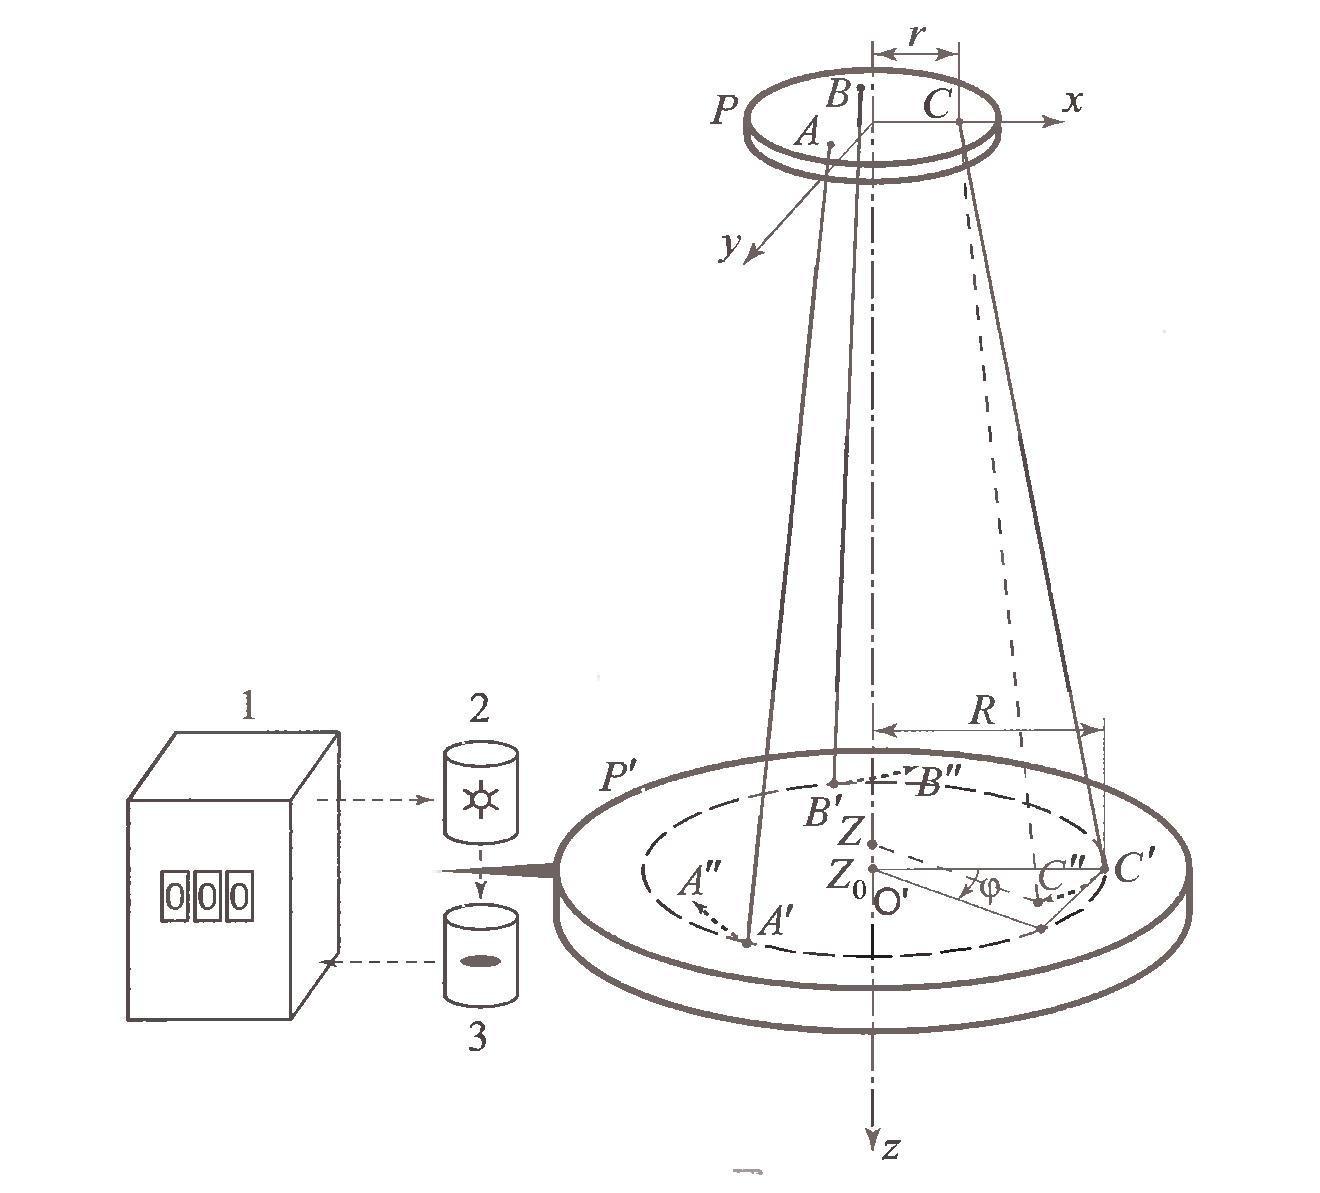
\includegraphics[width=0.4\textwidth]{123.jpg}
    	\caption{Трифилярный подвес}
    	\label{ris:trifilar}
	\end{wrapfigure}
	
	
	\begin{flushleft}
		\begin{spacing}{1.6}
		
Момент инерции твердого тела относительно неподвижной оси определяется по формуле: $ I = \int r^2 dm $.\\
Для однородных тел известной плотности при заданных размерах и достаточно простой форме момент инерции можно легко посчитать. Для неоднородных тел и тел слоной формы момент инерции можно поределить экспериментальною. Для этого удобно использовать устройство, называемое трифилярным подвесом. Оно состоит из укрепленной на некоторой высоте неподвижной платформы $P$ и подвешенной к ней на трех симметрично расположенных нитях $AA'$, $BB'$, $CC'$ вращающейся платформы $P'$.\\
Путем небольшого поворота верхней платформы можно возбудить крутильные колебания в системе. Уравнение сохранения энергии при колебаниях можно записать в виде:
\begin{equation}	
\frac{I\ddot{\varphi}^2}{2} + mg(z_{0} - z) = E
\label{equ:first}	
\end{equation}			
			
В системе координат, связанной с верхней платформой, координаты верхнего подвеса нити $C$ равны $(r, 0, 0)$. Нижний подвес нити в равновесии является точкой $C'(R, 0, z_{0})$, а при повороте платформы на угол $\varphi$ эта точка перейдет в $C''(R\cos\varphi, R\sin\varphi, z)$. Расстояние между точками $C$ и $C''$ равно длине нити $L$. Так, что:
\begin{equation}
(R\cos\varphi- r)^2 + R^2\sin^2\varphi + z^2 = L^2
\label{equ:second}	
\end{equation}

Учитывая малость угла $\varphi$:
\begin{equation}		
z^2 = L^2 - R^2 - r^2 + 2Rr\cos\varphi \approx z^2_{0} - 2Rr(1 - \cos\varphi) \approx z^2_{0} - Rr\varphi^2
\label{equ:third}	
\end{equation}

Решая (\ref{equ:third}):
\begin{equation}
z = \sqrt{z^2_{0} - Rr\varphi^2} \approx z_{0} - \frac{Rr\varphi^2}{2z_{0}}
\label{equ:fourth}	
\end{equation}
			
		\end{spacing}
	\end{flushleft}
	
		Подставляя данное уравнение в ЗСЭ и дважды дифференцируя по времени, после сокращений, получаем:
		
	\begin{equation}
		 I\ddot{\varphi}^2 + mg\frac{Rr}{z_{0}}\varphi= 0
		 \label{equ:fifth}	
	\end{equation}
	
	
		Решая уравнение (\ref{equ:fifth}) относительно $\varphi$, получаем:
			
	
	\begin{equation}
		\varphi = \varphi_{0}\sin\left(\sqrt{\frac{mgRr}{Iz_{0}}}t + \theta\right)
		\label{equ:sixth}
	\end{equation}
	
	
	Из (\ref{equ:sixth}) следует, что:
	
	\begin{equation}
		T = 2\pi\sqrt{\frac{Iz_{0}}{mgRr}}		
	\end{equation}
	
	\begin{equation}
		I = kmT^2, \qquad k = \frac{gRr}{4\pi^2z_{0}}
		\label{equ:seventh}
	\end{equation}

	\newpage	

\section{Выоплнение работы.}

	\subsection{Проверка установки.}
		
		\qquad  Перед началом выполнения лабораторной работы, выполним проверку установки. Для этого, возбудим крутильные колебания нижней платформы и определим время затухания. Установку будем считать исправной, если время затухания $$\tau \gg T$$
		
		Для удобства наблюдения, определим, за какое время амплитуда колебаний платформы (угол отклонения от начального положения) уменьшиться в 2 раза.
      В нашем случае, измерения проводить будем при значении амплитуды $15^{\circ}$.
		
	
		
		\subsection{Определение параметров установки.}
		Мы работали на установке №7. Запишем в таблицу информацию о нашей платформе
		\begin{table}[h!]
			\begin{center}
			\begin{tabular}{| l | l | l | l |}
					\hline
					m г & R мм & r мм & L см \\ \hline
					993.5$\pm$0.5 & 115$\pm$0.5 & 30.5$\pm$0.3 & 217.5$\pm$0.1 \\
					\hline
				\end{tabular}
			\end{center}
			\caption{Параметры платформы.}
			\label{tab:parametrs}
		\end{table}
		
Сразу заметим, что различие между $z_{0}$ и $L$ меньше погрешности.	Поэтому дальше будем считать их равными...	
		
		
		\subsection{Определение момента инерции установки.}
 Наш рабочий диапазон$-$когда период не зависит от амлитуды колебаний (заметим, что при весьма малых значениях амплитуды эта зависимость вновь проявляется). Для нашей установки походящее значение амплитуды равно $15^{\circ}$.
\par Проведем измерения времени десяти колебаний при таком значении амплитуды. Из этих данных определим период колебаний нашей платформы и её момент инерции:

\begin{table}[ht!]
	\begin{center}
	\begin{tabular}{|c|c|c|c|c|c|c|c||c|c|}
		\hline
		$t_{10}$ с & 44.036 & 44.013 & 44.010 & 44.007 & 43.967 & 43.966 &  43.990 & $T = 4.399c$ &$\delta T = 0.001c$\\
		\hline
	\end{tabular}
    \caption{Время колебаний пустой платформы.}
	\end{center}
	\end{table}
Отсюда момент инерции установки: $I=\frac{T^2mgRr}{4\pi^2z_{0}}\Rightarrow I=(7.69\pm 0.11)\cdot10^{-3}$ $kgm^{2}$.
	
	
	
	
	
	  \subsection{Определение момента инерции заданных тел. Проверка аддитивности момента инерции.}

          \begin{table}[ht!]
	\begin{center}
	\begin{tabular}{|c|c|c|c|c||c|c|}
		\hline
		$t_{10}$ с & 39.724 & 39.608 & 39.588 & 39.540 & $T_{disk} = 3.961c$ &$\delta T_{disk} = 0.001c$\\
		\hline
	\end{tabular}
    \caption{Крышка на платформе.}
	\end{center}
	\end{table}

          \begin{table}[ht!]
	\begin{center}
	\begin{tabular}{|c|c|c|c||c|c|}
		\hline
		$t_{10}$ с & 42.708 & 42.647 & 42.592 & $T_{ring} = 4.264c$ &$\delta T_{ring} = 0.001c$\\
		\hline
	\end{tabular}
    \caption{Кольцо на платформе.}
	\end{center}
	\end{table}

          \begin{table}[ht!]
	\begin{center}
	\begin{tabular}{|c|c||c|c|}
		\hline
		$t_{10}$ с & 40.054 & $T_{ring+disk} = 4.005c$ &$\delta T_{ring+disk} = 0.001c$\\
		\hline
	\end{tabular}
    \caption{Кольцо+Крышка. Проверка аддитивности.}
	\end{center}
	\end{table}

		\begin{table}[ht!]
			\begin{center}
			\begin{tabular}{| p{65pt} | p{110pt} | p{100pt} |}
					\hline
					Тело & Период колебаний, с & Масса груза, г \\ \hline
					платформа &4.399 & 993.5 \\ \hline
					платформа, Крышка & 3.691 & 584.4+993.5=1577.9 \\ \hline
					платформа, Кольцо & 4.264 & 821.1+993.5=1814.6 \\ \hline
					платформа, Кольцо+Крышка & 4.005 & 2399 \\
					\hline
				\end{tabular}
			\end{center}
			\caption{Периоды колебаний и параметры различных тел на трифилярном подвесе.}
			\label{tab:periods_diff_body}
		\end{table}

Проверка аддитивности момента инерции$\Leftrightarrow$проверке выполнения равенства $I_{ring+disk}=I_{ring}+I_{disk}-I$. Вычислим моменты инерции всех тел используя формулы (\ref{equ:seventh}). Занесём результаты в общую таблицу (\ref{tab:moments}) моментов инерции. И посмотрим: \textbf{есть ли аддитивность?}

  		\begin{table}[h!]
			\begin{center}
				\begin{tabular}{| l | c |}
				\hline
				Тело & Момент инерции, $kg*m^{2}, * 10^{-3}$ \\ \hline
				Платформа & 7.69 \\ \hline
				Платформа, Крышка & 8.61 \\ \hline
				Платформа, Кольцо & 13.21 \\ \hline
				Платформа, Кольцо+Крышка & 15.04 \\ \hline
				\end{tabular}
				\caption{Моменты инерции различных тел.}
				\label{tab:moments}
			\end{center}					
		\end{table}

\par Из полученного видно, что желаемое соотношение для моментов инерции выполнено, а значит наше утверждение об аддитивности моментов инерции доказано.

\subsection{Проверка закона Гюйгенса-Штейнера.}
Теперь разберемся с двумя "половинками". Разместим их на платформе как показано на рисунке \ref{ris:position}. Далее будем мерять время десяти полных колебаний, смещая после каждого такого измерения полудиски на расстояние $h=5$мм. В результате измерений мы получим зависимость $T(h)$, а затем, используя формулу \ref{equ:seventh}, получим $I(h^2)$. Результаты занесём в соответствующие таблицы.
	    \begin{wrapfigure}[10]{r}{0.29\textwidth}
			\vspace{-3em}
			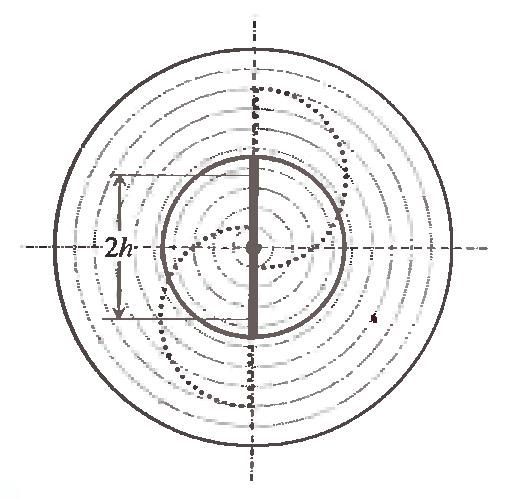
\includegraphics[width=0.25\textwidth]{position.jpg}
			\caption{Расположение тел на платформе.}
			\label{ris:position}
		\end{wrapfigure}	

\begin{table}[b]
			\begin{center}
				\begin{tabular}{| l | l || l | l || l | l || l | l ||}
					\hline
					№ изм. & $t_{10}$  с & T  с & h  см & № изм. & $t_{10}$  с & T  с & h  см\\ \hline
					1 & 30.545 & 3.054 & 0 & 8 & 34.435 & 3.443 & 3.5 \\ \hline
					2 & 30.712 & 3.071 & 0.5+x & 9 & 35.459 & 3.545 & 4.0 \\ \hline
					3 & 30.764 & 3.076 & 1.0 & 10 & 36.349 &3.635 & 4.5 \\ \hline
					4 & 31.154 & 3.173 & 1.5 & 11 & 37.645 & 3.764 & 5.0 \\ \hline
					5 & 32.048 & 3.205 & 2.0 & 12 & 38.981 & 3.898 & 5.5 \\ \hline
					6 &  32.819& 3.282 & 2.5 & 13 & 39.994 & 3.999 & 6.0 \\ \hline
					7 & 33.532 & 3.353 & 3.0 & 14 & 41.322 & 4.132 & 6.5 \\ \hline
				\end{tabular}
				\caption{Зависимость периода колебаний от расстояния между "половинками".}
				\label{tab:period}
			\end{center}
		\end{table}
Массы этих самых половинок (дисков) равны 764.5 г. Отсюда посчитаем моменты инерции и выведем зависимость.
\begin{table}[t]
			\begin{center}
				\begin{tabular}{| l | l | l || l | l | l |}
					\hline
					№ изм. & I, $kgm^2 * 10^{-3}$ & h, cm & № изм. & I, $kgm^2 * 10^{-3}$ & h, сm \\ \hline
					1 & 6.563 & 0 & 8 & 8.343 & 3,7 \\ \hline
					2 & 6.637 & 0,52 & 9 & 8.844 & 4,2 \\ \hline
					3 & 6.658 & 1,2 & 10 & 9.298 & 4,7 \\ \hline
					4 & 7.085 & 1,7 & 11 & 9.971 & 5,2 \\ \hline
					5 & 7.229 & 2,2 & 12 & 10.693 & 5,7 \\ \hline
					6 & 7.581 & 2,7 & 13 & 11.254 & 6,2 \\ \hline
					7 & 7.912 & 3,2 & 14 & 12.016 & 6,7 \\ \hline
				\end{tabular}
				\caption{Зависимость Момента инерции от расстояния между "половинками".}
				\label{tab:moment}
			\end{center}
		\end{table}
\newpage
\begin{minipage}[h]{0.69\textwidth}
\begin{tikzpicture}[scale = 1]
\begin{axis}[
    axis lines = left,
    legend style={at={(0.9, 0.3)}},
    xlabel = {$h^2$, $cm^2$},
    ylabel = {$I\cdot10^{-3}$, $kgm^2$},
    xmin=0, xmax=50,
    ymin=6, ymax=14,
	ymajorgrids = true,
	xmajorgrids = true
]
\addplot[
	mark = square, 
	mark options = {
		scale = 1.5, 
		fill = red, 
	},
	ymajorgrids = true,
	xmajorgrids = true,
	color = blue 
]  coordinates {
	(0, 6.563) (0.25, 6.637) (1, 6.658) (2.25, 7.085) (4, 7.229) (6.25, 7.581) (9, 7.912) (12.25, 8.343) (16, 8.844) (20.25, 9.298) (25, 9.971) (30.25, 10.693) (36, 11.254) (42.25, 12.016)};

\addplot [
    domain=0:100, 
    samples=1000, 
    color=red,
]
{6.563+x*0.129};

\legend{ 
	Experiment,
	Theory
};
\end{axis}
\end{tikzpicture}
\end{minipage}
\newpage		

 \subsection{Определение момента инерции диска, его массы.}
Из таблицы \ref{tab:moment} определим момент инерции диска на платформе. Он отвечает значению $h=0$ то есть $I=6.563$ $kgm^2$.\\
Теперь из формулы (\ref{equ:seventh}) определим массу диска.
\begin{displaymath}
M=\frac{I}{kT^2}=\frac{4\pi^2z_{0}I}{gRrT^2}\Rightarrow M= 1757
\end{displaymath}
\textbf{Теперь вычтем из $M$ 993.5 г.$-$ массу платформы, получим 763.5 г.} Видим, что различие с истинным значением всего лишь 1 грамм, то есть $\sim0.13\%$.\\
Аналогично для кольца:\\
 $I_{ring exp}=(13.21-7.69)\cdot10^{-3}=5.52\cdot10^{-3}$ $kgm^2$\\
$m_{ring exp}=820$г.


      \subsection{Определение момента инерции тел с использованием теоретических формул и сравнение размеров тел.}
Определим, совпадают ли полученные значение моментов инерции с теоретическими. Измеренный диаметры диска \textbf{87.9}мм.
	
		Для этого, используем следующие формулы:
		
		\newpage
		
		\begin{flushleft}
			\begin{spacing}{1.6}
				$ I_{disk} = \frac{1}{2}mR^2 $
				
				$ I_{ring} = \frac{m}{2}(R_{int}^2 + R_{ext}^2)$
			\end{spacing}
		\end{flushleft}
		
		Подставив в данные формулы значения $ m_{disk th}=764.5$г, $ R_{disk th}=\frac{87.9}{2} $мм, $ m_{ring th}=821.1$г, $ R_{ring ext}=83.6$мм, $R_{ring int}=78.5$мм. Тогда получаем:		
		
		\begin{flushleft}
			\begin{spacing}{1.6}
				$ I_{disk th} =0.738 \cdot 10^{-3}  \quad kgm^2 $
				
				$ I_{ring th} =5.40 \cdot 10^{-3}  \quad kgm^2 $
			\end{spacing}
		\end{flushleft}

В силу доказанной аддитивности момента инерции $I_{disk+platform}=I_{disk exp}+I_{platform}$, где:\\
$I_{platform}=7.69\cdot 10^{-3}$ $kgm^2$.\\
$I_{disk+platform}=6.563\cdot 10^{-3}$ $kgm^2$.\\
Экспериментальное значение момента инерции диска:\\
\begin{spacing}{1.6}
$I_{disk exp}=(7.69-6.563)\cdot10^{-3}=1.127\cdot10^{-3}$ $kgm^2$
\end{spacing}
Отсюда экспериметальное значение радиуса диска: $R_{disk exp}=\sqrt{\frac{2I_{disk exp}}{m_{disk exp}}}\Rightarrow R=54.3$мм.\\
Разница с реальным радиусом (44мм) составляет 23.5\%.\\

Экспериментальное значение момента инерции диска:\\
$I_{ring exp}=5.52\cdot10^{-3}$ $kgm^2$\\
Упрощенно найдем экспериментальное значение радиуса кольца:\\
$R_{ring exp}=8.2$ $cm$. Что крайне близко к истинному значению(98\%).

      \subsection{Определение погрешностей измерений.}	 
Погрешность $k$:
\begin{flushleft}
			\begin{spacing}{1.4}
				$ \sigma_{k} = k\sqrt{\left(\frac{\sigma_{R}}{R}\right)^2 + \left(\frac{\sigma_{r}}{r}\right)^2 + \left(\frac{\sigma_{z_{0}}}{z_{0}}\right)^2} $

			   Подставляем  $\sigma_{R}=\sigma_{r}=\sigma_{z_{0}}=1mm\qquad$ 

				$ \sigma_{k} = 0.0136\approx0.01\qquad k \approx 0.40$
			\end{spacing} 
		\end{flushleft}
		
		Относительнаz погрешность измерения момента инерции:
		\begin{flushleft}
			\begin{spacing}{1.4}
				$ \varepsilon_{I} = \sqrt{\left(\frac{\sigma_{k}}{k}\right)^2 + 4\left(\frac{\sigma_{T}}{T}\right)^2} $
				$ \varepsilon_{I} = 0.089\Rightarrow\varepsilon_{I}=8.9\% $
			\end{spacing} 
		\end{flushleft} 
Тут мы приняли $\varepsilon_{T}\approx0.05$
		 
		\newpage		 
		 
\section{Вывод.}
\begin{enumerate}
\item Мы подтвердили аддитивность момента инерции. Все значения совпали в пределах погрешности.
\item Значение теоретического и экспериментального моментов инерции близки
\item Геометрические размеры тел определены не так точно, как хотелось бы, но результаты не очень различны.
\item Мы построили зависимость $I(h^2)$ и показали справедливость закона Гюйгенса-Штейнера. Зависимость очень близка к линейной.
\item Хотя у нас и возникли некоторые неточности в связи с тем, что мы не могли точно смещать бруски на одинаковую длинну $h$, но эту проблему вышло легко устранить. 
\end{enumerate}	


\end{document}
     